\section{Multi-Modal Policies}\label{sec:multi-modal-policies}

\subsection{Feature Level Fusion}\todo{really long intro, consolidate}
On top of just naively combining views (or modalities) and expecting the policy to understand what it means to `see' is a tall order. 

If these extracted features can be thought of as encoded information, as with latent representation models\todo{ref here and maybe mention earlier on the report}, multiple extractors will lead to to many encodings. So, the next challenge becomes merging; and not just how but when to merge features from one view to another. I will explain their potential positives and investigate the consequences of each.\todo[color=purple]{this might be a good segue or part in presentation}

\subsubsection{Early Fusion}
Fuse different modalities into a single input and run through the encoding model. This usually involves combining the raw data sources. Before any information is extracted or the data is modelled in any way.

Therefore, its advantages mostly lie in its simplicity. No dedicated processing has to be done per information stream. On the other hand, this can fall short of capturing complex interactions between these modalities; depending on the network and the semantic information each modality provides.

\subsubsection{Late Fusion}
This is the complete opposite of early fusion. Each modality will be run through its own model and predict a representation. The immediate advantage is that each model can learn a rich representation relating to only its given modality

\subsubsection{Intermediate Fusion}
This is the most common middle-ground. While separated feature learners can be used per desired modality, the representation extracted from them will be fused together. Then this aggregated latent representation can be passed through another model to get the final predictions. This is a tradeoff based system between early and late fusion. Most of the proposed systems will follow this idea.

\todo{i will argue separating the grasping network will be late fusion fuse at the actionn level and not separating it will be fully intermediate}

\section{Proposed Fusion Methods}\label{sec:proposed-fusion}
I designed a modular poly-policy which can be instantiated in any fusion configuration to handle its given modalities differently before making a final movement prediction. The modularity is within the `Feature Encoding' block shown in Figure \ref{fig:policies-skeleton-idea}\todo[color=blue]{maybe move to appendix}

\begin{figure}[htpb]
  \centering
  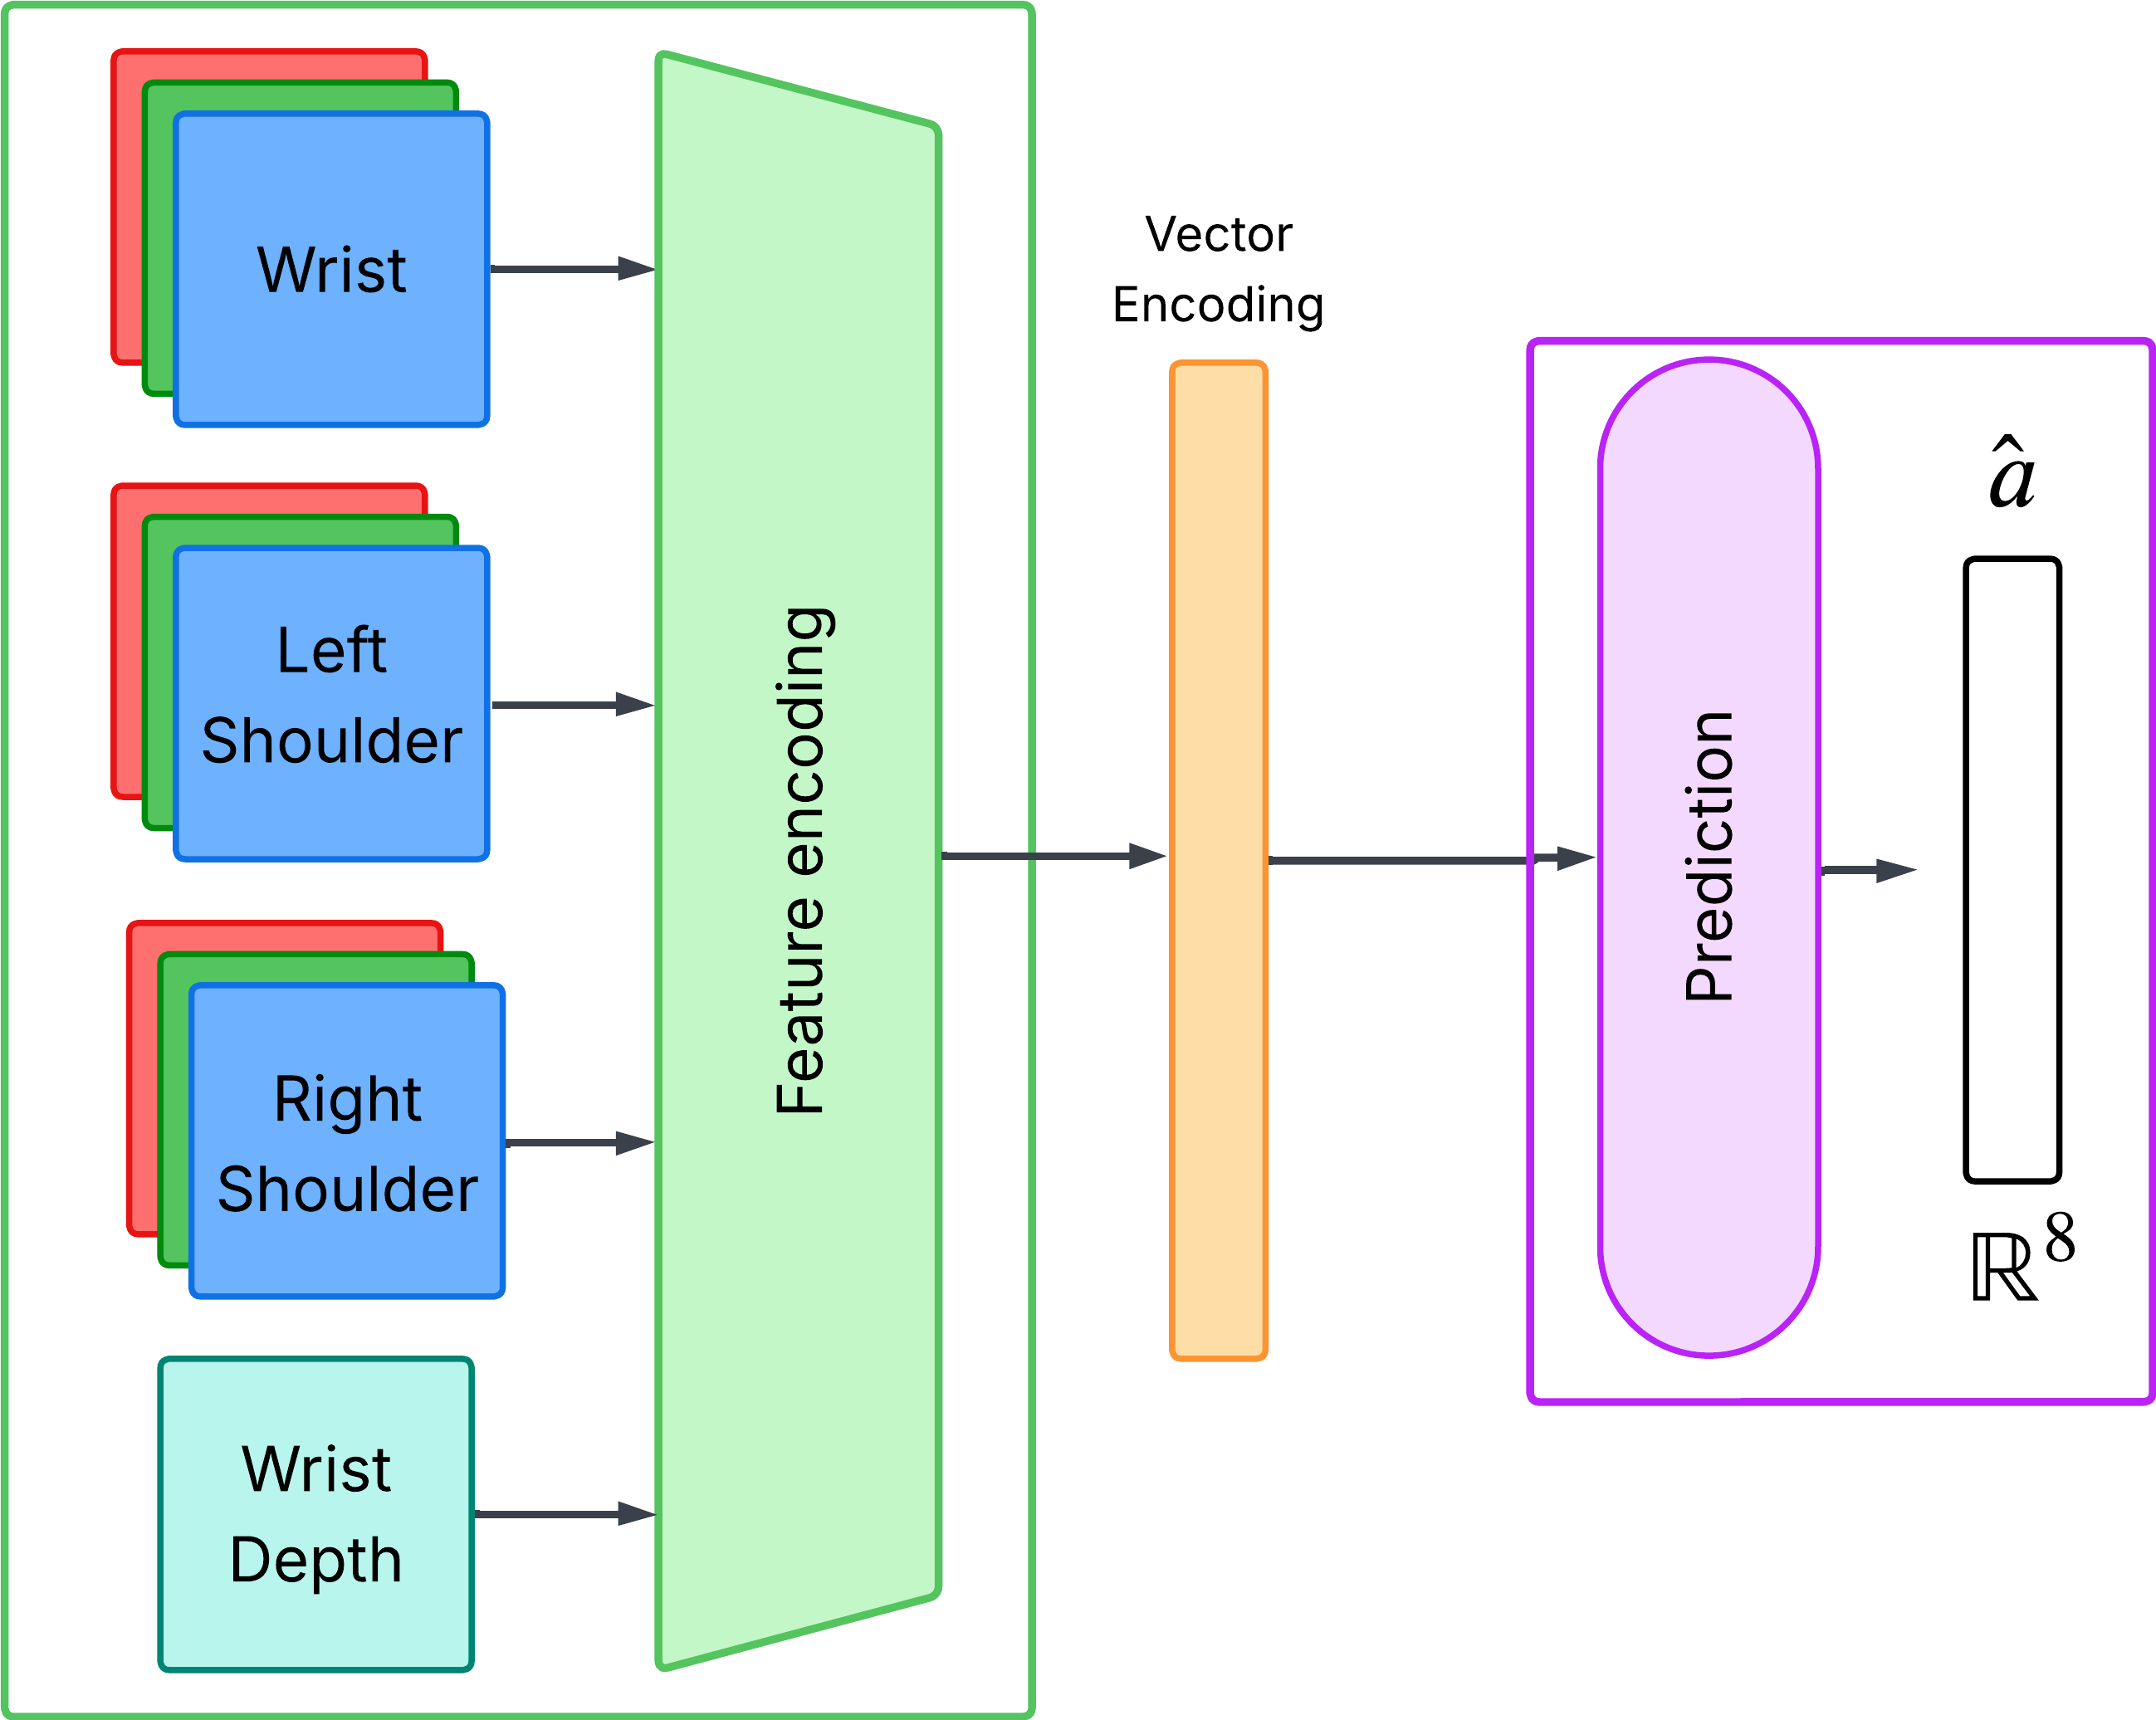
\includegraphics[width=0.2\linewidth]{assets/cam-comb/policies/general-diagram.png}
  \caption{Main Skeleton of the proposed policy structure}\label{fig:policies-skeleton-idea}
\end{figure}

\todo{add the fusingEncoder and the config to the appendix}
\subsection{Simple Stacking}
An example of early fusion, this is the naive method of just stacking the views on the channel dimension, and has clear disadvantages for this specific system.

Firstly, for the RGB cameras, there is definite misalignment, all these cameras have different poses and will disagree on what they see. Leading to features not lining up, leaving us with a non-optimal and more importantly a brittle\todo{explain brittle? or does the next senetence take care of it} policy. Meaning it could lead to unintended coupling of information which can lead to the agent making wrong choices during inference when the same views don't necessarily align during rollout.\todo{simple diagram of overlaid squares (arrow) model (arrow) representation} This will act as a baseline to compare other fusion strategies.

\subsection{Understanding Depth Separately}\label{subsec:policies-understand-depth-sep}
RGB provides a denser representation of the system and in a configuration with multiple RGB views the depth information may be drowned out. Therefore, an important first step was to learn the depth features separately and then make them influence the action. The idea here is to have a RGB encoder and a separate Depth encoder CNNs, then learn the best way to merge this data together. I propose three different methods to do this whish are highlighted in Figure \ref{fig:policies-sep-dep-diagrams}.

\begin{figure}[htpb]
  \centering
  \begin{subfigure}{0.45\linewidth}
    \centering
    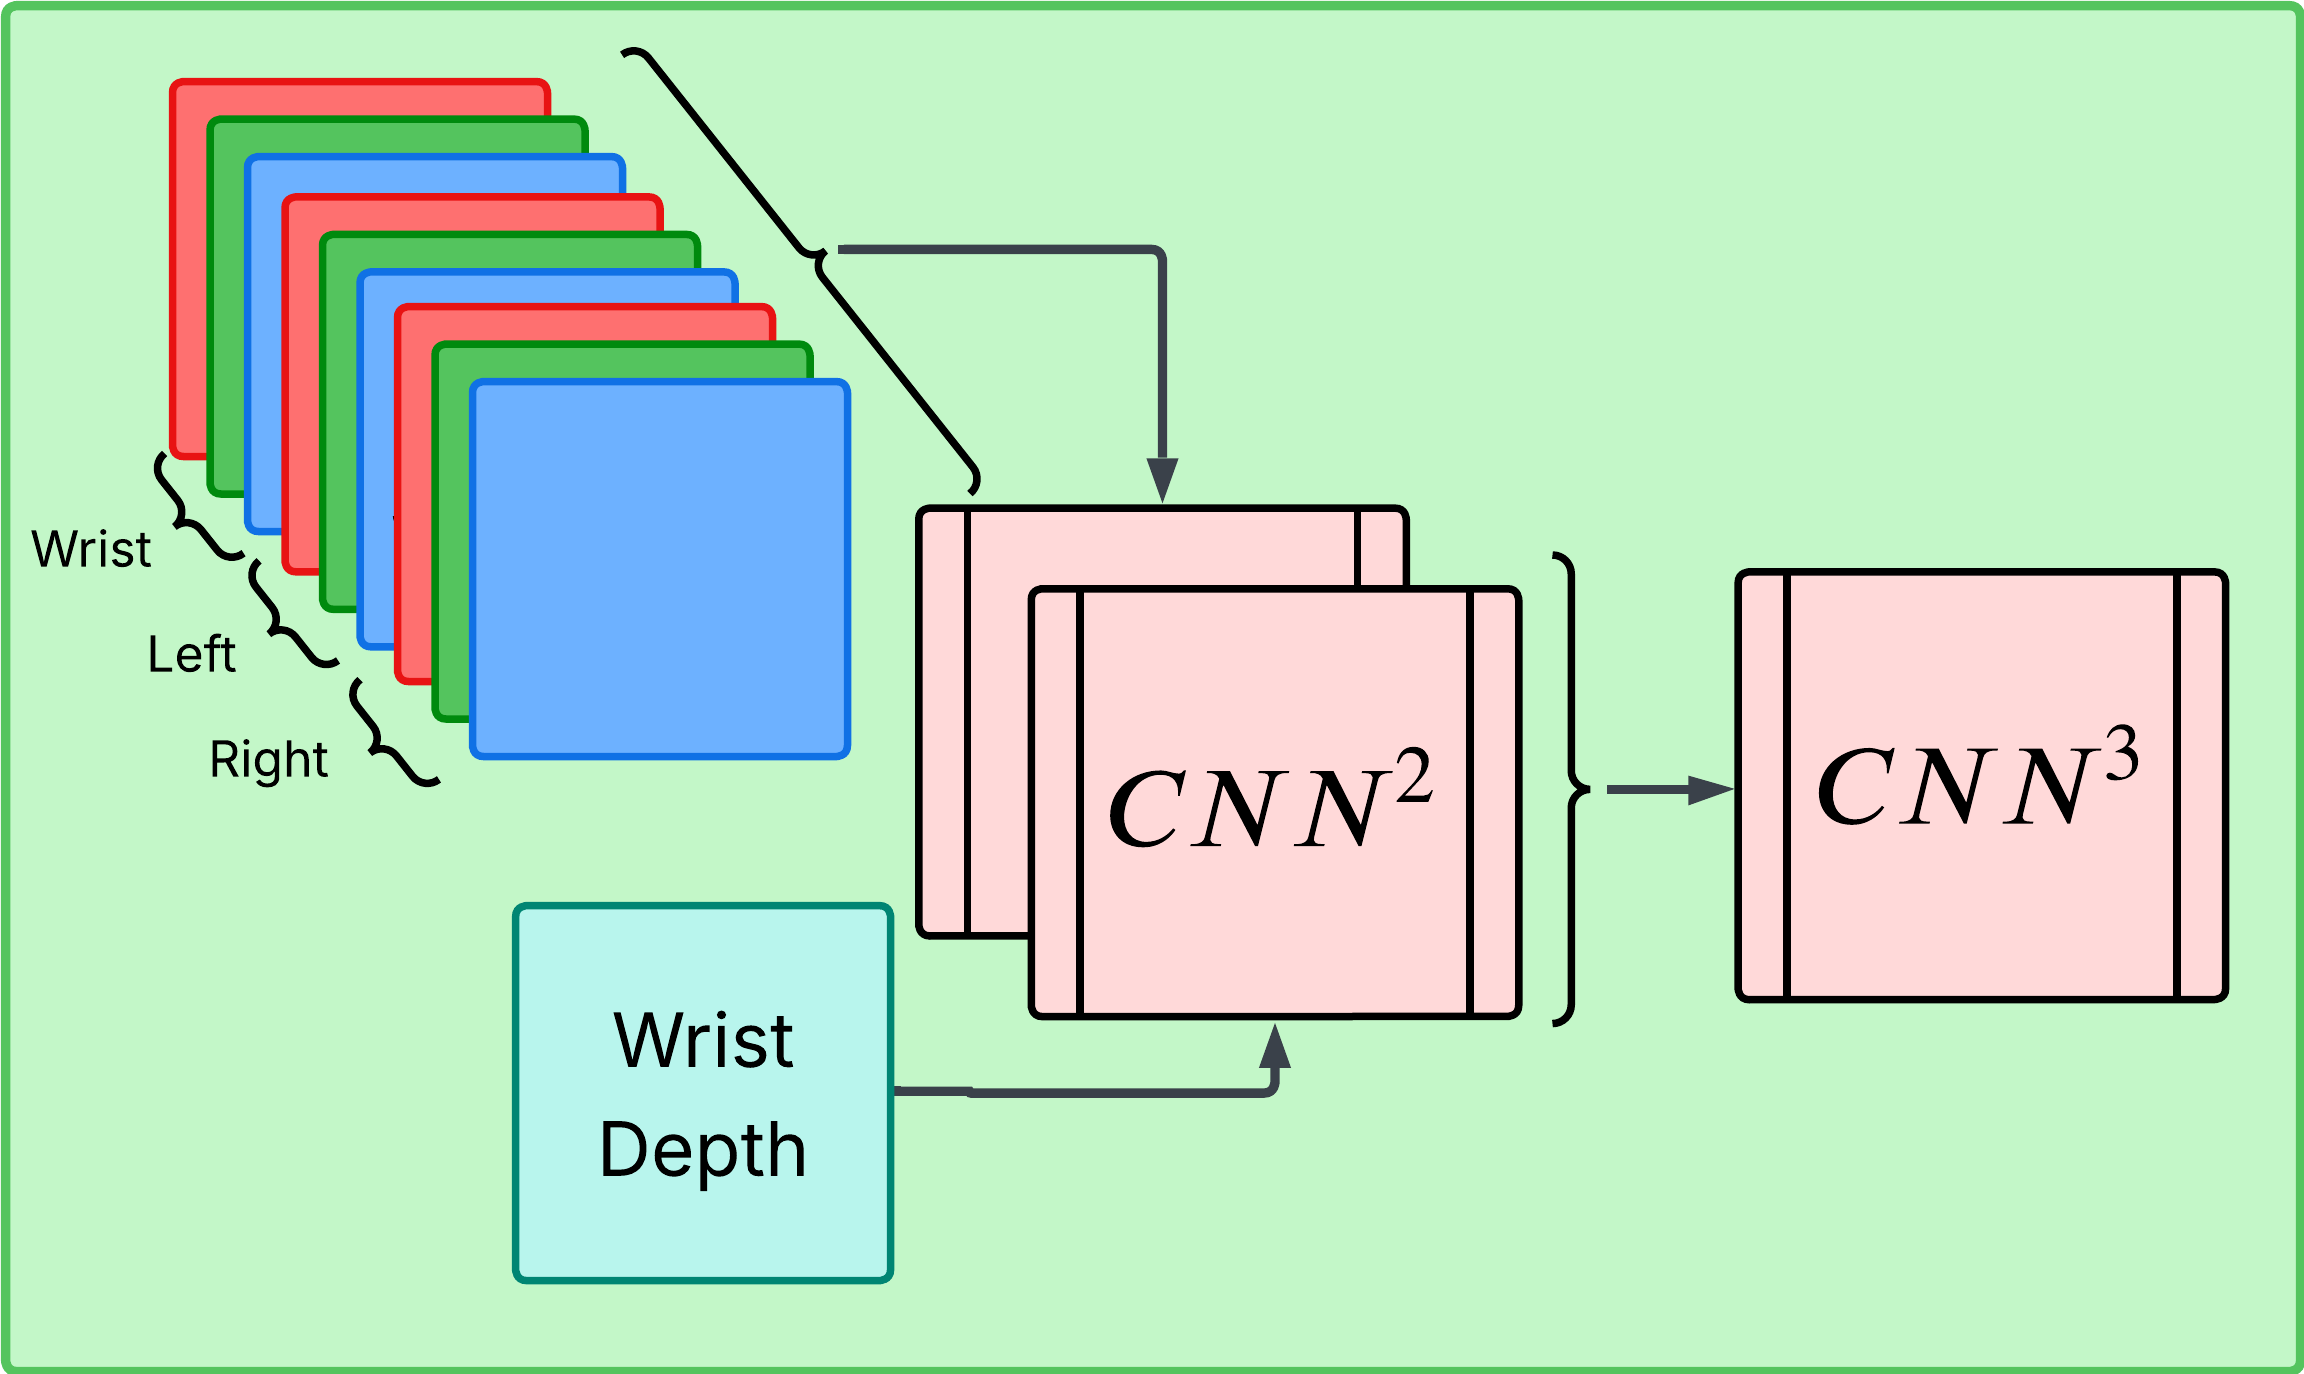
\includegraphics[width=0.5\linewidth]{assets/cam-comb/policies/wlr_d-feats-diagram.png}
    \caption{Simple concatenation of the features from each CNN}\label{subfig:policies-wlr_d}
  \end{subfigure}
  \hfill
  \begin{subfigure}{0.45\linewidth}
    \centering
    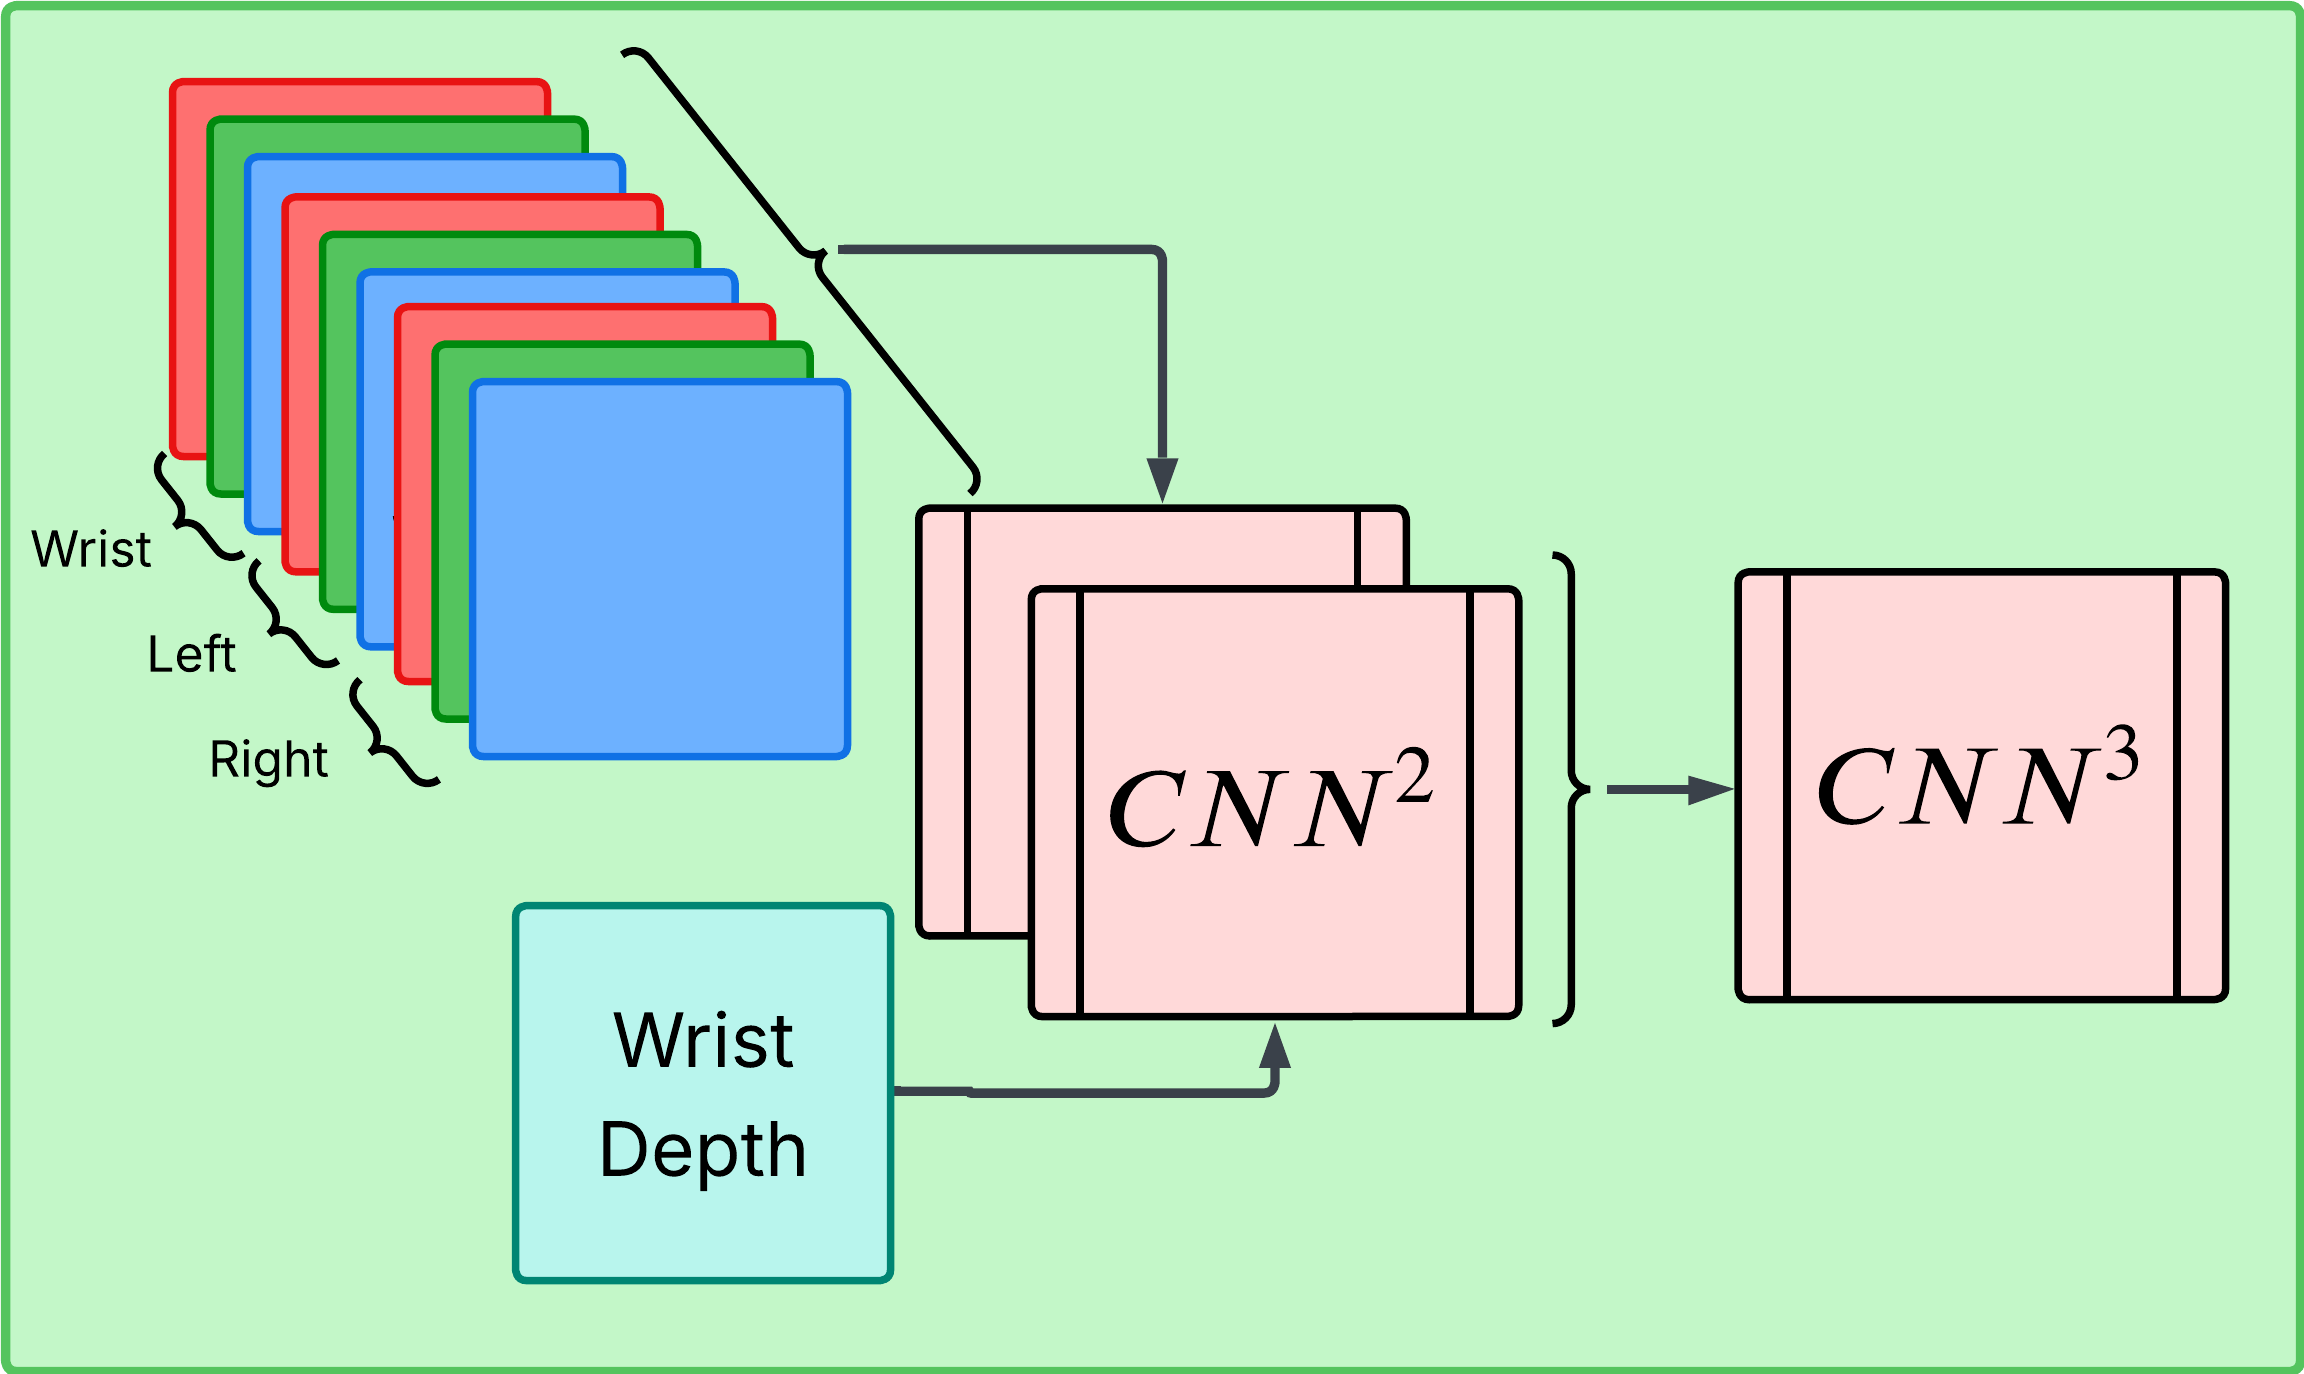
\includegraphics[width=0.5\linewidth]{assets/cam-comb/policies/wlr_d-feats-diagram.png}
    \caption{A second layer CNN, convolving the outputs in a learnable manner}\label{subfig:policies-wrl_d-feats}
  \end{subfigure}
  \vspace{0.5cm}
  \begin{subfigure}{0.45\linewidth}
    \centering
    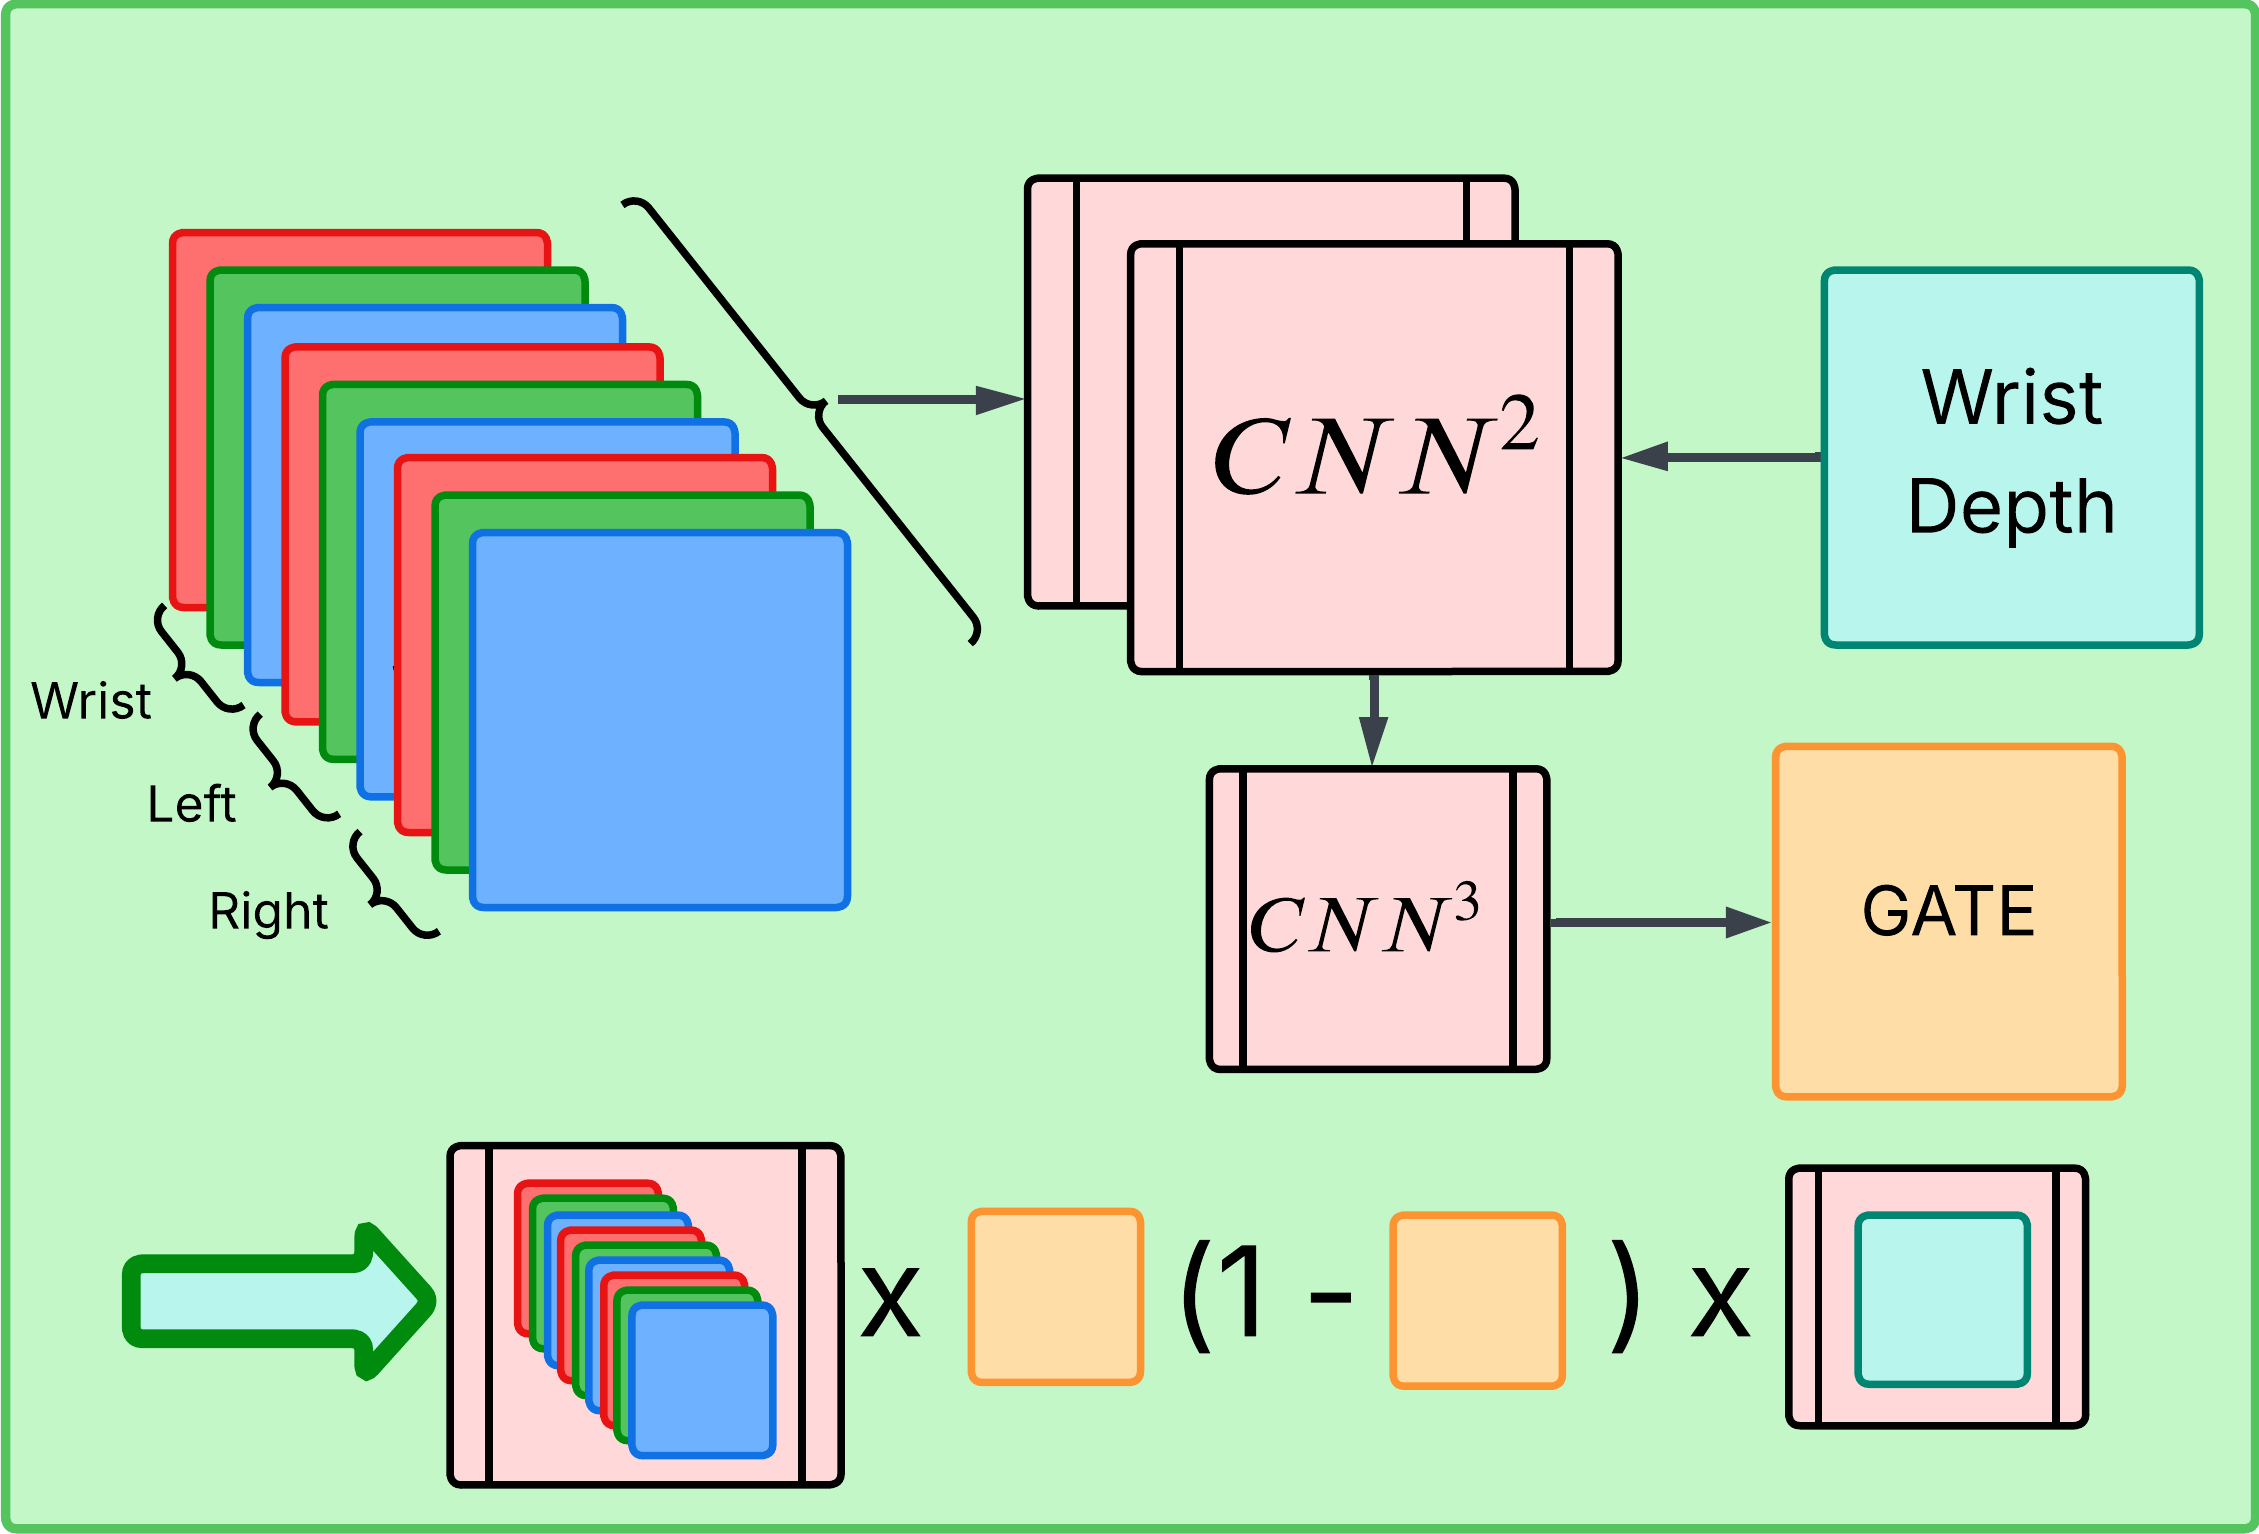
\includegraphics[width=0.5\linewidth]{assets/cam-comb/policies/wlr_d-gated-diagram.png}
    \caption{A shallower secondary CNN to learn simple \emph{gating} from already extracted RGB and Depth features.}\label{subfig:policies-wrl_d-gated}
  \end{subfigure}
  \hfill
  \begin{subfigure}{0.45\linewidth}
    \centering
    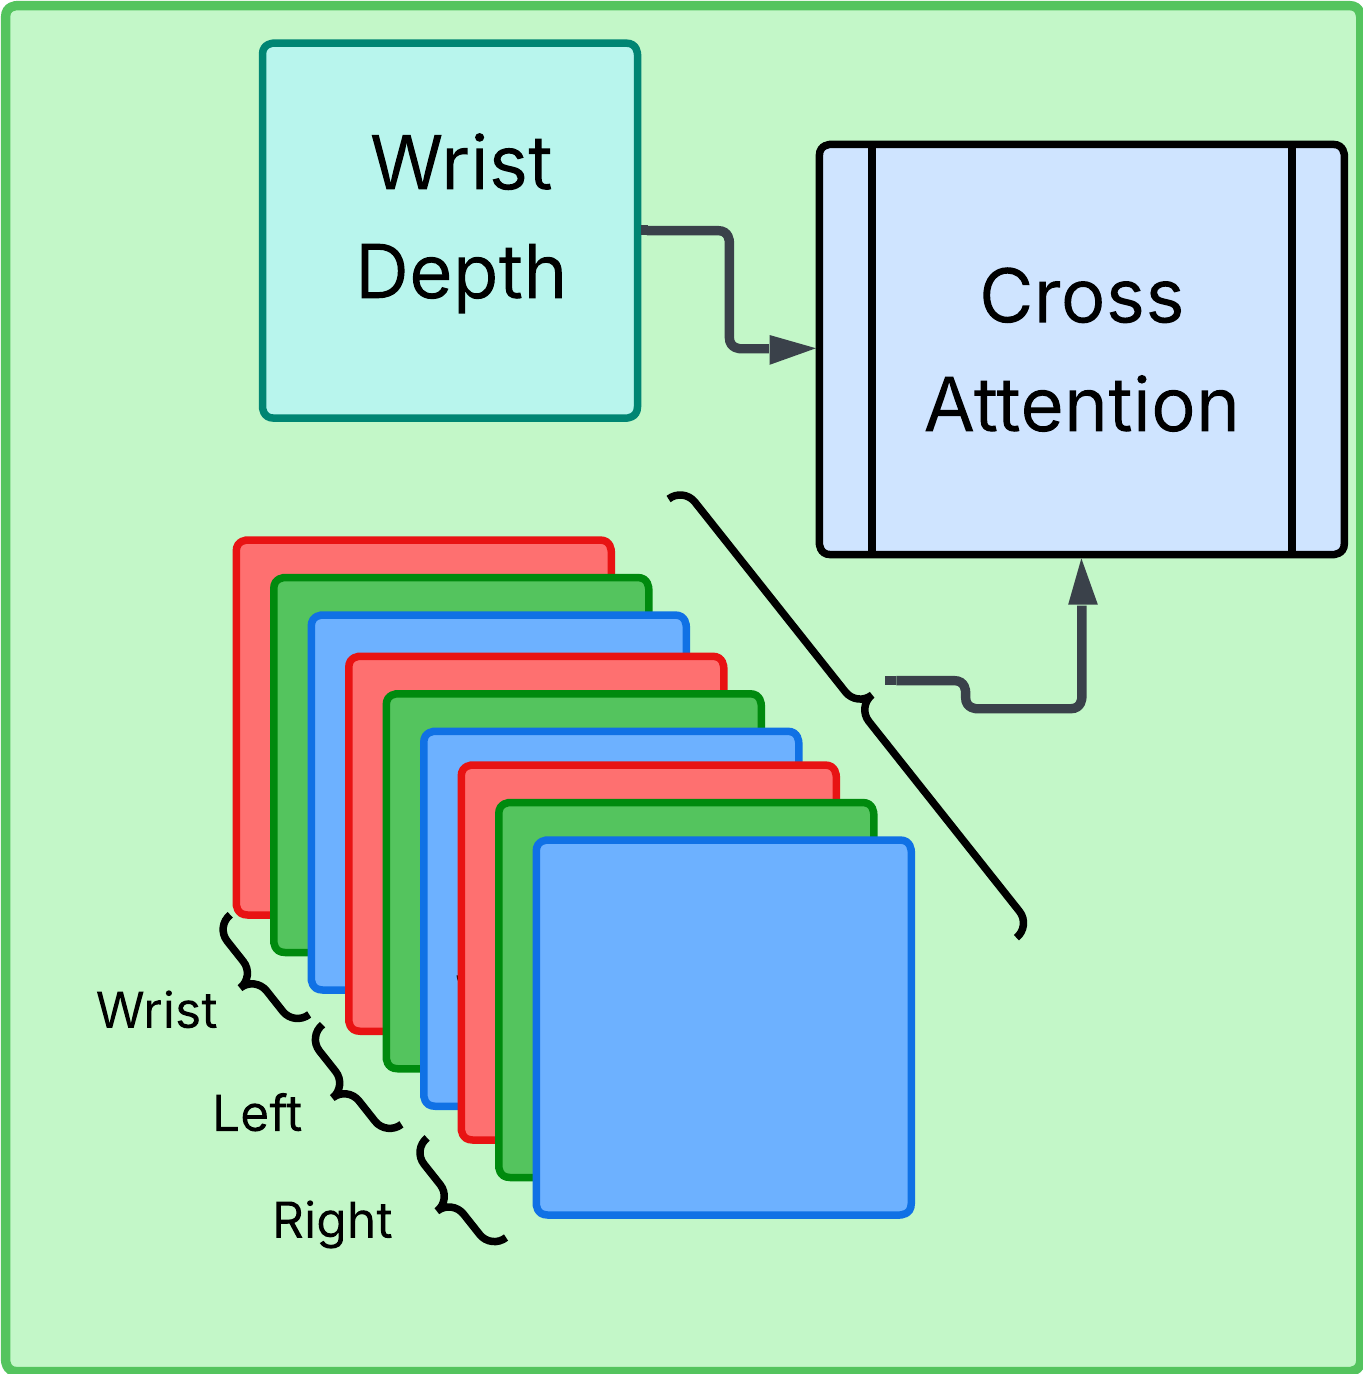
\includegraphics[width=0.5\linewidth]{assets/cam-comb/policies/wlr_d-attn-diagram.png}
    \caption{A Cross Attention Mechanism to attend to the important parts of from each extracted feature.}\label{subfig:policies-wrl_d-attn}
  \end{subfigure}
  \caption{Proposed Systems}\label{fig:policies-sep-dep-diagrams}
\end{figure}
Which are ultimately decoded into an \emph{action}, $\hat{a}$.

To elaborate \ref{subfig:policies-wrl_d-attn} further. the cross attention module takes in the the two modalities and firstly runs a small Conv to get to match their channels. Once matched to attend to features I used the Key-Query-Value attention \cite{vaswani2023attentionneed} between the two modalitiesm using the \verb|MultiHeadAttention| module \cite{pytorch}. Setting the query to the first modality and the key and value to the other modality I can get the score, \( a_{i, j} \propto \frac{Q_i^TK_j}/\sqrt{ch}\), I pass in 3D values and they are flattened before attention, so $ch$ is the original channel dimension after the first convolution, holding the encoded information about the modalities. After concatenating all the heads and running a softmax on the scores we will be able to get our output, which the score weighted `value' vector: \(\sum_{j}{{a'}_{i, j}v_j}\). The reason we set the value to our other modality is to `weight' it according how the first modality \emph{attends} to features in he second modality. The cross attention module I propose does it both ways. So, the RGB features will be weighted by Depth interactions and vice versa. Then similar to \ref{subfig:policies-wrl_d-feats} a learner CNN module will learn to distill this information down.\todo{shorten maybe not sure how this reads?}


\subsection{Feature-wise Linear Modulation}\label{subsec:policies-film}
To take a step back from all the excessive RGB data. I wanted to understand how modulating similar views with each other to understand similar observations from each other's perspective. Allowing the network to learn and discover its own trends is a fine task, however, implicitly injecting cues from modality into another will, in theory, allow the learning to be more efficient.

A light-weight and quick way to bias network parameters with conditional data is Feature-wise Linear Modulation (FiLM) \cite{perez2017film}. A FiLM network learns to adaptively influence the weights of another neural network by learning $f_c$ and $h_c$ as functions on the conditional input $\mathbf{x}_i$. So:

\[
\text{FiLM} = \left( \mathbf{F}_{i, c} | \gamma_{i, c}, ~\beta_{i, c} \right) = \gamma_{i, c}\mathbf{F}_{i, c} + \beta_{i, c} \qquad  \gamma_{i, c} = f_c\left(\mathbf{x}_i \right), \beta_{i, c} = h_c \left( \mathbf {x}_i \right)
\]
My implementation involves creating a simple linear network to generate the two parameters. So, my implementation of \(\phi\left(\mathbf{X}, \mathbf{Z}\right) = f\left(\mathbf{Z}\right)\mathbf{X} + h\left(Z\right)\) where $\mathbf{Z}$ is the modulator/condition, and $\mathbf{X}$ is the modulated modality. I defined $f$ and $h$ to be the two chunked parts of a linear network module, this means the parameters will have shared weights, which makes sense as the modulation is being conditioned on a single view, and hence a dependence between its scale and bias is expected. The 2D data is projected then pooled to handle the transitions between the dimensional differences.

I also initialise this network to be the identity modulation, meaning \(\gamma = 1 ~\text{and} ~\beta = 0\). This is helpful because it will stabilise the learning. Starting off with no modulation, it will respect the already aligned wrist and depth data. Then during training these cross-modal features will slowly fuse. And more importantly random a random initial bias might add suboptimal premature bias. Another inherent benefit is the network can be kept at a minimal size. This is one of the reasons to settle on a simple FiLM module compared to the likes of for example a cross-attention module as before. 

I created 3 different modulation configurations: wrist RBG modulated with wrist depth\todo{diagram}, depth modulated wrist RGB\todo{diagram}, and both modulated with each other\todo{diagram}. Where the modulated features act as the latent encoding, which can be used to predict an action as before.

A final positive, is that a FiLM module can be plugged in at multiple different places in the network at different scales. This allows for fine-tuning in when to modulate. For example, modulate on the raw inputs, run a cnn extract some high level features and modulate then, or wait to modulate later. As the resolution of my sensors is not too large I decided to do two configurations: early FiLM, where feature shapes are matched then modulated leading to a coarser scale modulation; also a finer version where the order of down-sampled learning and modulation are swapped, so modulations is done on the learnt representation of RGB and depth values.\todo{diagrams here}


\subsection{Derivative Methods}\label{subsec:derivative-methods}
The final propositions include 4-way fusion models that take into account ideas from earlier:
\begin{itemize}
  \item Fully separated feature extractors, all concatenated before action prediction \todo{add figure}
  \item Learning the wrist and shoulder groups separately. First with a naive CNN to fuse them, then an attention module as before to merge them.
  \item Pairwise FiLM between all modalities: wrist RGB and wrist Depth, then Left Shoulder RGB and Right Shoulder RGB; then concatenated before action prediction\todo{figre}
  \item Finally 4-way multi-modal cross-attention. \todo{add math and figure if needed}
\end{itemize}

These are all derived from the previous sections, and extending these ideas to all the sensors. Separating, all feature extractors allows us to learn representation for each, however it will place a lot of learning strain on the later decoder to give us a valid action. 

FiLM modules in theory are should be better at aligning already agreeable data, however would it be valid modulate the shoulders to each other and then to the modulated output of the wrist. This was mostly a curiosity, to see if there is a linear relationship that can be learnt between all the data streams.

And finally, 4-way cross attention. This is quite a promising system. The main idea is to patch the image into parts, and then run them through a vision transformer (ViT) along with positional information to attend to features within their own representation and also to each other. Creating a feature encoding, capsulating the relationship between regions of the sensors as well as the other sensor. \todo{more math about the positional encodings here etc} This is separate fron the attention system in \ref{subsec:policies-understand-depth-sep}, however, this accepts and all modality combinations and will take care of that. Although, I arbitrarily decided it should have at least two views, otherwise it would only do self attention, which might be useful in training, however, not contributing anything into fusion.

\subsection{Temporal Understanding of Demonstrations}
The actions in my system are heavily dependent on the context of where the robot came from. And the demonstrations contain coherent and smooth trajectories. Although, I am preserving the sequential nature of the demos in training. There is no implicit underlying mechanism to enforce the agent will learn from this. Due to the partially observable setting of my system, and the robot not knowing any extra information about its state (model-free), it is important to be able to keep a historical understanding of what has happened, or what the agent believes is important for that moment in time.

So, I incorporated recurrent models into the latent representation. This is so that the embedding of the current states will depend on a history of the earlier observations or states.
A pro of RNNs, compared making a bespoke sequential model is they are not length constrained \todo{was an earlier problem in 2d, maybe mention}. The sequences can be of any length which will help model the demos I have with varying episode lengths. Som compared to 3D CNNs \todo{ref}, which can also incorporate spatial and temporal information \todo{ref}


Another theoretical advantage is that the long-term memory can be used to have a \todo{mamybe mention the remoark from the then move test, }

\subsubsection{Latent RNN Encodings of Movement Steps}
To encode timestep information into my already existing features, I added an Long-Short Term Memory (LSTM), which is a type of Recurrent Neural Network (RNN) \todo{cite} network module near the end of the pipeline\todo{add figure}. Meaning the history will be kept in the latent space.

So, this simple idea of introducing temporal noise into the decision process, should in theory allow for more concise predictions that are grounded in what the agent has observed so far. I kept the design modular so that any flavour of feature fusion from above can then be fed through this RNN, allowing the encoding of latent fused embeddings to then be temporally learnt.

\subsection{ViT Time-Stamped Encodings}\todo{kind of dabled with this but will not be testing it}
\todo[color=red]{not done much on this, but may be able to talk about how I would go about it or just remove}
A similar idea to the RNN method above was to do a full vision transformer similar to \ref{subsec:derivative-methods}, but on top of positional encodings to denote the image patch, I was also going to encode temporal information of where in the sequence that frame came from. Following a very natural language processing (NLP) approach to transformers.\todo{ref here}

\todo{talk about the implementation of this in math maybe a diagram}



\subsection{Proprioception}\todo{maybe talk about why I left it out earlier in the chapter}
Up until this point, I left proprioceptive data out of the training, mainly because I wanted to train on purely visual feedback to see what it could achieve without any other state information. Secondly, including state information about the robot, would not necessarily immediately help with the task learning. \todo{quick explanation of proprio data and maybe a diagram}

To investigate I created a simple feature projection network. That takes in the $7$-dimensional joint position data and learns to project it to a higher dimension, to add to the extracted view features before the final movement decision. The main benefit of this, it gives us a modular system that can be attached to any of the other systems for quick testing. As most parts of this system.

\subsection{Numerical Foundations}\todo{talk about the general math, like what are the shapes of the data, what is the loss minimising-maximising, and notation}

The policies above are trained in the same way and the only separation is the modular feature extraction blocks, as well as what data they require. All input and output is handled within the network and the policy interface exposed to the agent is compatible with all the ones proposed in this project.

\subsubsection{The Dataset}
A demonstration of episode length $T$ is defined as: \(\mathcal{D} := \{\langle o_t, ~a_t\rangle\}_{t = 1}^{T} \). Observation, \(o_t \in \mathcal{O}\) is defined as the available modalities to the system with shape \(\mathcal{O} := \mathbb{R}^{c \times W \times H}\). This corresponds the resolution of the sensor (\textbf{W}idth and \textbf{H}eight) also $c \in \left[1, 10\right]$ which correspond to the available modality data concatenated on their channel dimension. The order of $c$ is always:\todo{figure here with the stuff stacked}
\[
{RGB}_{wrists}, ~{RGB}_{{left}\_{shoulder}}, ~{RGB}_{{right}\_{shoulder}}, ~{Depth}_{wrist}
\] 
where the $RGB$ data is $3$ channels wide while $Depth$ is only 1. \(a_t \in \mathbb{R}^{8 \times 1}\) is the corresponding joint velocities at timestep $i$, which acts as our ground truth. 

The Data Loader, as discussed \todo{ref}, will provide a randomly shuffled batch of $b$ collated demos, along with extra information. \( \langle O^B, ~A^B, ~\left( P^B, ~l^B \right) \rangle\), where \(O^B \in \mathbb{R}^{ B \times c \times W \times H}\). The observation batch size, $B$ is equal to \({\sum_{ d \in \mathcal{D}^B}|d|}\), this is the sum of the length of all demos in this training batch. Similarly, \(A^B \in \mathbb{R}^{B \times 8}\) per joint velocity (7) and final grasp indicator, \(P^B \in \mathbb{R}^{B \times 7}\) per joint angle - the proprioception data. Finally, \(l^B \in \mathbb{Z}^{b}\), contains the original lengths of the individual demos.

Then during the forward pass modalities of interest will be extracted from $O^B$ and features will be extracted depending on what fusion flavour is picked.



\subsubsection{Fine-Grained per Time-Step Training}\todo[color=green]{math fixing}
The RNN policy is disconnected from the main system.\todo{link the FusionRNNPolicy appendix} Differently from above, the batched demonstrations will now respect the individual lengths of provided demonstrations. The loader will now emit: \( \langle {O'}^B, ~{A'}^B, ~\left( {P'}^B, ~l^B \right) \rangle\). The \emph{prime} ($'$) indicates a change in their batch dimesion, each now follow $\mathbb{R}^{b \times T_{max} \times \ldots}$ and  $T_{max}$ is the longest demonstration in this batch \(\max l^{B}\). We pad every demo to this length while keeping the original lengths $l^{B}$.

To fit the network to our data quite closely I opted to train the network with information at every step. Meaning every single step $i$ in a demo $mathcal{D}$ with episode length $T$, will have an action predicted with respect to $\mathcal{D}_{t < i}$ and will have an impact on the loss of the system. 

The loss will be calculated using the predicted actions, $\hat{A}$ and the ground truth labels, $A$; as \( \mathcal{L}^{action} = {loss}_{mse}\left(A_{x, t} - \hat{A}_{x, t}\right)\) for $x$ being the batch number in $1..b$ and $t$ the timestep in $1..T_{max}$. A bit mask \(M \in \{0, 1\}^{b \times T_{max}}, ~M_{x, t} = 1, ~t < l^B_x ~else ~0\) will be used to only extract the loss items lying withing the sequence lengths of demos. Finally, the loss per epoch will be normalised by the number of timesteps in the demos provided. \(loss = \frac{1}{\sum_{x, t}M_{x, t}}{\sum_{x = 1}^{b}\sum_{t = 1}^{T_{max}}M_{x, t} \mathcal{L}^{action}}\)

As before\todo{ref to earlier grasp}, the grasping loss is separated in the default configuration of this policy. Giving the final loss as: 
\[
  \mathcal{L}^{action} = \mathcal{L}^{pose} + \lambda_{grasp} \mathcal{L}^{grasp}
\]
where $\mathcal{L}^{pose}$ and $\mathcal{L}^{grasp}$ are calculated using the same masking method as above.

\missingfigure{updated diagram to convey the padding and unpacking and training the loss on every frame step}


\section{Moving to \emph{Active Vision}}
End-to-end models with absolutely zero fine-grained interactions are quite competent. However, in the chaotic and random environments an agent may be acting in. Planning and specific nudges may prove beneficial. Similar to the 

\todo{improve the grasping}

\todo{It might be worth scaling everthing to 128 by 128 next week and do a repeat run so that I can at least say that I have done it}

\todo{ruun grasp then move and confirm the suspicions of the policies with no memory failing.}